\documentclass[a4paper,10pt]{article}
\usepackage[utf8]{inputenc}
\usepackage{xspace}
\usepackage{graphicx,graphics} 


%opening
\title{Algorithmic model for N-GREEN optical ring}




\begin{document}

\maketitle
\section*{Problem}
The application we study takes place in the C-Ran context. We want to centralise calculations into a common data-center for an area of antennas distributed on the territory. The data between the RRH (antennas) and the BBU (data-center) are transiting through an optical ring. We study here only the behaviour of the ring. First, for an easier model, we consider a ring in which one or two nodes are the data-centers, and the other nodes of the ring sends some data coming from the RRH.

Every millisecond, between each couple RRH-BBU, the following periodic process is observed:
\begin{enumerate}
 \item The RRH sends some latency critical data to its BBU.
 \item Those data are transferred to the BBU through the ring .
 \item After a computation time of the message, the BBU sends an answer to its RRH.
\end{enumerate}
 This periodic process has a critical end to end latency, thus a messages has to be as little buffered as possible before being sent in the ring.
 Every messages will browse the entire ring during the process. Since the ring is approximately 50km long, a messages needs $250 \mu s$ to travel this length.
 Considering that the periodicity of the emissions ($1ms$) is greater than a ride of the ring, we take $P$ a multiple of the time needed to travel the ring.
 
 
 
\section*{Sending policy}
In the studied model, the nodes of the ring have a {\bf broadcast and select} policy. Then, the physical times needed to insert the data in the ring are negligible in regard of the other times.
When a node sends a packet on the ring, it contains data for several destinations. Every node of the ring reads all the slots and keep the data addressed to it. It copy the data of the packet in the slot, but does not remove anything. The only node that can free a slot is the one which send a packet in it.

%when a node sends some data in a slot, this slot is {\em taken} by this node for an entire ride of the ring. This means that every nodes of the ring can collect the information addressed to it, but it does not delete the data in the slot. The slot is fully cleared by the node that sent it, when it came back after a ride of the ring.


Thus, a node has to wait for a free slot before sending a packet in the ring. To avoid overloading the ring, a node sends a packet only if some criteria  are satisfied.
We define by $Q$ the capacity of the buffer of a node, $\alpha$ the {\em minimum load} of the buffer, $0 \leq  \alpha \leq 1$, and $\delta$ the {\em maximum delay}.

The node sends a packet in a slot if:
\begin{itemize}
 \item The amount of data $q$ in the buffer is greater than $\alpha . Q$,
 \item or the older data in the buffer is waiting for more than $\delta$.
\end{itemize}

The buffer of a node is filled with the FIFO rule by a traffic coming from external sources. Then, when the node has an available free slot, the packet is inserted in the slot if one of the previous constraints are satisfied. Otherwise the node does not send anything in the ring and wait for the next free slot.

\begin{center}   

      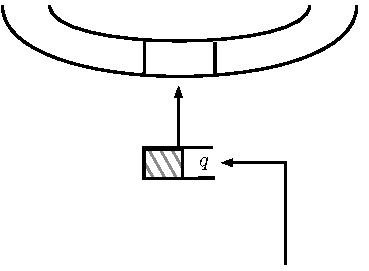
\includegraphics[scale=0.7]{insertion0.pdf}

  
\end{center}

\section{C-RAN context}

In C-RAN context, this amount of data $q$ contains two kinds of data: the latency critical flow coming from RRH or BBU, and an other flow, called {\em best effort}.

We can consider two buffers containing $x$ and $y$ amount of data. The first one is filled with the C-Ran data in priority, and the best effort flow if needed, the second one takes the rest of best effort flow. We consider that, even if a lot of RRH are represented by a node on the ring, the amount of C-Ran data incoming to a node is strongly lower than the capacity of a packet ($\simeq 1.2$ Gbps for each RRH, 100 Gbps into the ring).
The C-RAN data comes periodically in regard of the period $P = 1ms$. 
The best effort data comes more randomly (can be modelled by a Poisson distribution, for example), and are inserted in the buffer if $x = 0$.

\begin{center}   

      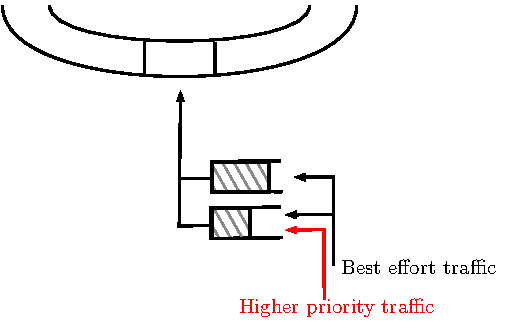
\includegraphics[scale=0.7]{insertion1.pdf}

  
\end{center}
 
 
\section*{Model}
We consider an optical ring composed of $k$ nodes ($k={3,...,10}$).
We are in a discrete time model: the time is split in $N$ slot, rotating to the following position each time step $t = 10 \mu s$. This value is the switching granularity.
\begin{center}   

      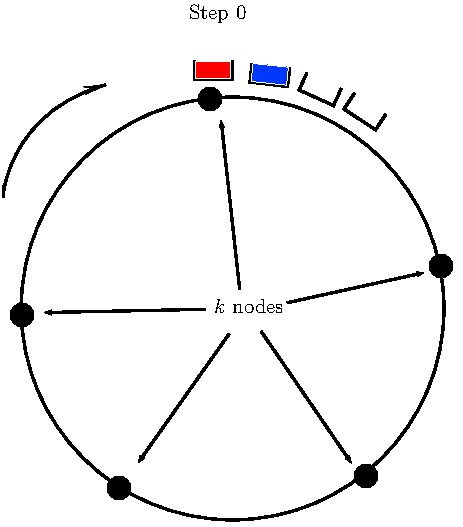
\includegraphics[scale=0.5]{anneau1.pdf}
      \hspace{3cm}
      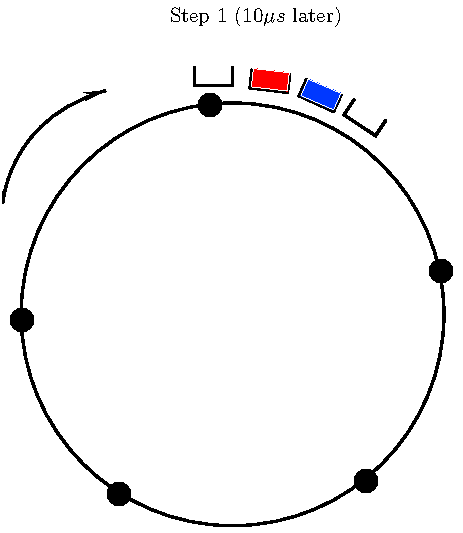
\includegraphics[scale=0.5]{anneau2.pdf}
  
\end{center}

Considering a length of 50 km for the ring, we evaluate the number of slots about 25 into the ring.

\section*{Study}
The purpose is here to reduce the latency of the C-RAN data. Two event can increase this latency: 
\begin{enumerate}
  \item The node has enough data $q$ to emit in the ring, but no slots are available.
 \item The node does not have enough data $q$ to emit and a data from $x$ is waiting for less than $\delta$.
\end{enumerate}

In a first time, we will look at the first problem, and try to determine from what load of the ring, the time taken to wait a free slot in the ring is too long.



\end{document}